\begin{surferPage}{巴斯六次曲线}
1996年,沃尔夫巴斯构造了这个六次曲面。巴斯六次曲面有65个奇异点。杰夫 与 卢德曼后来证明了巴斯六次曲面是奇异点最多的六次曲面--所以巴斯的世界纪录是无懈可击的!
巴斯曲面的出现对人们来说是一个巨大的惊喜,因为曾经在相当长的一段时间里,人们误以为六次曲面只能有64个奇异点。
巴斯曲面具有一个非常好的性质:二十面体对称性。下图展示的是一个二十面体以及它的一个对称平面。

  \begin{center}
    \vspace*{-0.1cm}
    \begin{tabular}{@{}c@{\ \ }c@{\,}c@{}}
      \begin{tabular}{@{}c}
        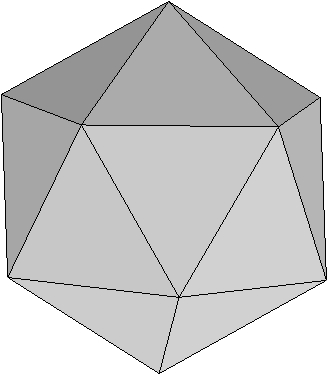
\includegraphics[width=1.4cm]{icosah}
      \end{tabular}
      &
      \begin{tabular}{@{}c}
        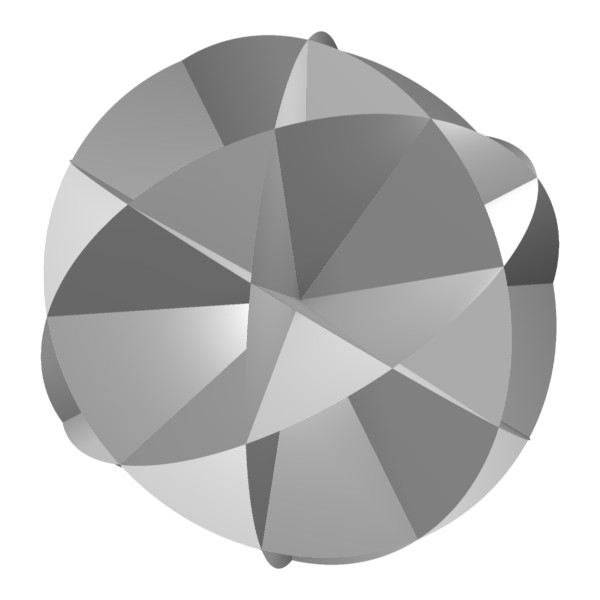
\includegraphics[width=1.4cm]{barth_sextic_planes}
      \end{tabular}
      &
      \begin{tabular}{c@{}}
        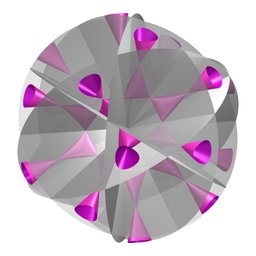
\includegraphics[width=1.4cm]{barth_sextic_and_planes}
      \end{tabular}
    \end{tabular}
  \end{center}
  \vspace*{-0.1cm}

巴斯六次曲面满足方程 $P_6 - \alpha K^2=0.$ 其中 $P_6$表示六个对称平面, $K=x^2+y^2+z^2-1$ 是单位球面, 并且
    $\alpha=\frac{1}{4}(2+\sqrt{5})$.
\end{surferPage}
